\section{Experiments}

We have implemented and trained our SAMNet model using MI-Prometheus~\cite{kornuta2018accelerating}, a framework based on Pytorch~\cite{paszke2017automatic}. 
We evaluated the model on the COG dataset~\cite{yang2018dataset}, a video reasoning~\cite{mogadala2019trends} dataset developed for the purpose of research on relational and temporal reasoning.
Our experiments were designed to study SAMNet's performance as well as its generalization abilities in different settings.
For this purpose, we used two different variants of the COG dataset (\cref{tab:cog_variants}): an easy one (Canonical) and a Hard version to explore a wide range of difficulties.
The main differences are the number of frames in the input sequence (4 vs. 8) and the maximum number of distractors (i.e., objects not relevant for the answer) per a single frame (1 vs. 10).


\begin{table}[htb]
\caption{Details of the Canonical and Hard variants of the COG dataset}
\centering
\begin{tabular}{lcccccc}
	\toprule
	Variant    &  	number &  	maximum & maximum & size & size & size  \\ 
	& of   & memory & number of & of & of & of  \\
	& frames & duration & distractors & training set & validation set & test set \\
	\midrule
	Canonical & 4 & 3 & 1 & 10000320 & 500016? & 422400? \\	
	Hard  & 8 & 7 & 10 & 10000320 & 500016?  & 422400? \\
	\bottomrule	
\end{tabular}
\label{tab:cog_variants}
\end{table}


%More details on the dataset, its variants and tasks can be found in the Appendix.


%
%We compare our model to the original COG model  ~\cite{yang2018dataset} using their implementation (https://github.com/google/cog) and scores given by the authors. We also use the exact same training parameters detailed in the original paper.
%
%On the other side we trained SAMNet using IBM's Mi-Prometheus~\cite{kornuta2018accelerating}, a framework for research based on Pytorch. We trained all our models using NVIDIA’s GeForce GTX TITAN X GPUs. We trained  SAMNet using 8 reasoning steps SAMCells and a hidden state size of 128. The external memory has 128-bit slots. We trained our model until convergence but we also have set a training time limit of 80 hours.

\subsection{Performance comparison with the COG baseline}

In our experiments we have trained SAMNet using 8 reasoning steps and external memory having 8 address locations, each being a vector of 128 floats.
We have also carried out experiments with different numbers of reasoning steps and memory size, but this goes beyond the scope of this paper.
In here, we have focused on 22 classification tasks and compared our results with the baseline model.
The most important results are highlighted in~\cref{fig:samnet_cog_detailed}, whereas full comparison is presented in \cref{tab:results-full}.

\begin{figure}[htbp]
	\centering
  \begin{subfigure}{\textwidth}
    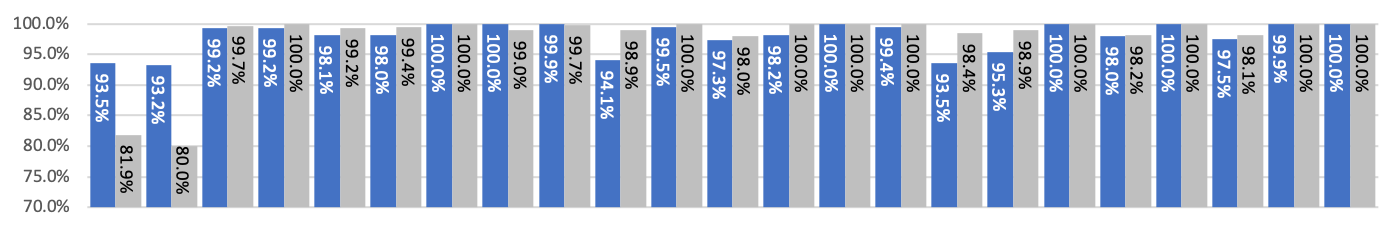
\includegraphics[width=0.99\textwidth]{../results/samnet_cog_orig_canonical_no_labels.png}
  \end{subfigure}%
  \newline
  \begin{subfigure}{\textwidth}
	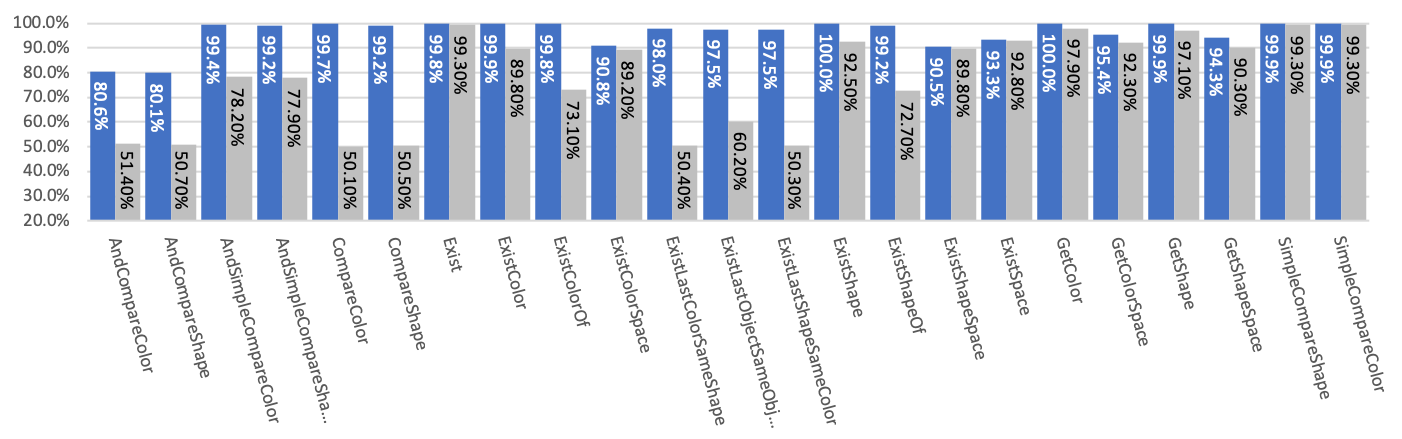
\includegraphics[width=\textwidth]{../results/samnet_cog_orig_hard.png}
  \end{subfigure}%
\caption{Comparison of test set accuracies of SAMNet (blue) with original results achieved by the COG model (gray) on Canonical (top) and Hard (bottom) variants of the COG dataset.}
\label{fig:samnet_cog_detailed}
\end{figure}


For the Canonical variant (top row), we have achieved similar accuracies for the majority of tasks (with the total average accuracy of 98.0\% in comparison of 97.6\% achieved by the COG model), with significant improvements (around 13 points) for \textit{AndCompare} tasks.
As those tasks focus on compositional questions referring to two objects, we hypothesize that our model achieved better accuracy due to the ability to selectively pick and store the relevant objects from the past frames in the memory.
Despite there are some tasks in which our model reached slightly lower accuracies,
% (between 0.2 and 1.8 points)
when comparing performances on the Hard variant, it dominates COG baseline on all tasks, with improvements varying from 0.5 to more than 30 points.

\begin{table}[t!]
\caption{COG test set accuracies for SAMNet \& COG models. Below `paper' denotes results from~
	while `code' denotes results of our experiments using their implementation~\cite{yang2018implement}}
\centering
\begin{adjustbox}{width=\textwidth}
\begin{tabular}{lcccccccccc}
	\toprule
	Model & & SAMNet & && && COG&& \\
	\cmidrule{2-5} \cmidrule{7-11} 
	&&&&& & paper & ours & ours & paper&\\
	\cmidrule{7-9} \cmidrule{10-11}
	Trained on       & canonical & canonical & canonical & hard &           &  canonical  & canonical  & canonical & hard \\ 
	Fine tuned on  & - & - & hard  & - &           & -   & - & hard & - \\ 
	Tested on        & canonical & hard & hard & hard &            &canonical  & hard & hard & hard  \\ 
	\midrule
	
	Overall accuracy & 98.0 & 91.6 & 96.5  & 96.1 &           & 97.6  & 65.9 & 78.1& 80.1 \\ 
	
	\midrule 
			
	AndCompareColor			&	93.5	&	82.7	&	89.2	&	80.6	&	&	81.9	&	57.1	&	60.7	&	51.4	 \\
	AndCompareShape			&	93.2	&	83.7	&	89.7	&	80.1	&	&	80.0	&	53.1	&	50.3	&	50.7 \\
	AndSimpleCompareColor		&	99.2	&	85.3	&	97.6	&	99.4	&	&	99.7	&	53.4	&	77.1	&	78.2 \\
	AndSimpleCompareShape		&	99.2	&	85.8	&	97.6	&	99.2	&	&	100.0	&	56.7	&	79.3	&	77.9 \\
	CompareColor			&	98.1	&	89.3	&	95.9	&	99.7	&	&	99.2	&	56.1	&	67.9	&	50.1 \\
	CompareShape			&	98.0	&	89.7	&	95.9	&	99.2	&	&	99.4	&	66.8	&	65.4	&	50.5	 \\
	Exist				&	100.0	&	99.7	&	99.8	&	99.8	&	&	100.0	&	63.5	&	96.1	&	99.3 \\
	ExistColor			&	100.0	&	99.6	&	99.9	&	99.9	&	&	99.0	&	70.9	&	99	&	89.8 \\
	ExistColorOf			&	99.9	&	95.5	&	99.7	&	99.8	&	&	99.7	&	51.5	&	76.1	&	73.1 \\
	ExistColorSpace			&	94.1	&	88.8	&	91.0	&	90.8	&	&	98.9	&	72.8	&	77.3	&	89.2 \\
	ExistLastColorSameShape		&	99.5	&	99.4	&	99.4	&	98.0	&	&	100.0	&	65.0	&	62.5	&	50.4 \\
	ExistLastObjectSameObject	&	97.3	&	97.5	&	97.7	&	97.5	&	&	98.0	&	77.5	&	61.7	&	60.2 \\
	ExistLastShapeSameColor		&	98.2	&	98.5	&	98.8	&	97.5	&	&	100.0	&	87.8	&	60.4	&	50.3 \\
	ExistShape			&	100.0	&	99.5	&	100.0	&	100.0	&	&	100.0	&	77.1	&	98.2	&	92.5 \\
	ExistShapeOf			&	99.4	&	95.9	&	99.2	&	99.2	&	&	100.0	&	52.7	&	74.7	&	72.70 \\
	ExistShapeSpace			&	93.4	&	87.5	&	91.1	&	90.5	&	&	97.7	&	70	&	89.8	&	89.80 \\
	ExistSpace			&	95.3	&	89.7	&	93.2	&	93.3	&	&	98.9	&	71.1	&	88.1	&	92.8 \\
	GetColor			&	100.0	&	95.8	&	99.9	&	100.0	&	&	100.0	&	71.4	&	83.1	&	97.9 \\
	GetColorSpace			&	98.0	&	90.0	&	95.0	&	95.4	&	&	98.2	&	71.8	&	73.	&	92.3 \\
	GetShape			&	100.0	&	97.3	&	99.9	&	99.9	&	&	100.0	&	83.5	&	89.2	&	97.1	 \\
	GetShapeSpace			&	97.5	&	89.4	&	93.9	&	94.3	&	&	98.1	&	78.7	&	77.3	&	90.3 \\
	SimpleCompareShape		&	99.9	&	91.4	&	99.7	&	99.9	&	&	100.0	&	67.7	&	96.7	&	99.3 \\
	SimpleCompareColor		&	100.0	&	91.6	&	99.80	&	99.9	&	&	100.0	&	64.2	&	90.4	&	99.3 \\
	\bottomrule
\end{tabular}
\end{adjustbox}
\label{tab:results-full}
\end{table}


\begin{wrapfigure}{r}{0.5\textwidth}
	\centering
	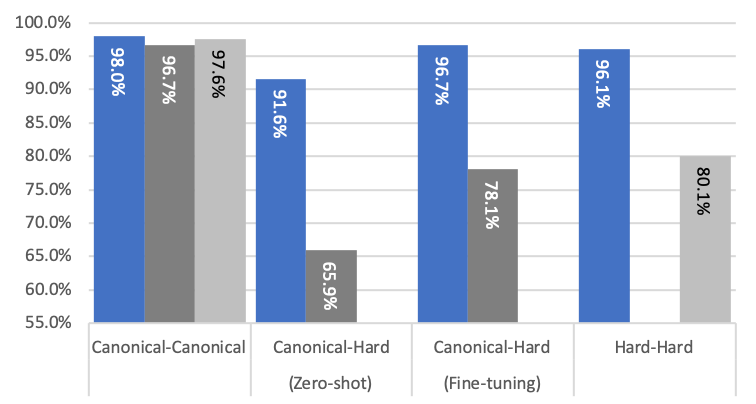
\includegraphics[width=0.5\textwidth]{../results/samnet_cog_overall_transfer.png}
	\caption{Total accuracies of SAMNet (blue) and COG models (light/dark gray) when testing generalization from Canonical to Hard variants of the dataset.}
	\label{fig:samnet_cog_overall_transfer}
\end{wrapfigure}

The goal of the next set of experiments was to test the generalization ability concerning the sequence length and number of distractors.
For that purpose, we have compared the accuracies of both models when trained on the Canonical variant and tested on Hard (\cref{fig:samnet_cog_overall_transfer}).
As the original paper does not include such experiments, we have performed them on our own.  The light gray color indicates the original results, whereas dark gray indicates the accuracies of COG models that we have trained (fine-tuning/testing) using the original code provided by the authors.
For sanity check, in the first column, we report both the best-achieved score and the score reported in the paper when training and testing on Canonical variant, without any fine-tuning.
In a pure \textit{transfer learning} setup (second column), our model shows enormous generalization ability, reaching 91.6\% accuracy on the test set.
We have also tested both models in a setup where the model trained on a Canonical variant underwent additional fine-tuning (for a single epoch) on the Hard variant (third column).
In this case, the SAMNet model also reached much better performance, and, interestingly, achieved better scores from the model trained and tested exclusively on the Hard variant.
In summary, the results clearly indicate that the mechanisms introduced in SAMNet  enable it to learn to operate independently of the total number of frames or number of distractions, and allow it to generalize to longer videos and more complex scenes. One other strength of SAMNet is its interpretability. Observing attention maps (see Appendix) shows that SAMNet can effectively perform multi-step reasoning over questions and frames as intended. It also accurately classifies temporal contexts as designed. However we notice that the model can sometime discover alternative strategies that were not in the intended design but the answers are still correct. More details are given in the Appendix.

%we used the canonical (easy) and hard settings that alter the number of distractors and sequence length.  Since there was no baseline for these tests (train on canonical, test on hard), we ran our own experiments using the COG model provided by the authors.  SAMNet achieves the highest overall scores for all categories of experiments (\cref{fig:samnet_cog_overall_transfer}), especially for the tests run on the hard dataset.  Among the 22 classification tasks, we highlighted the two most difficult tasks that affect the overall score. 
%We argue that the generalization capability of SAMNet is mainly due to the dynamic frame-by-frame processing of the input sequence. 
%The mechanisms introduced in SAMCell learn to operate independently of the total number of frames and allow to generalize to longer video lengths.
%As shown in \cref{fig:samnet_cog_overall_transfer}, when trained on the easy dataset, SAMNet still performs 91.6\% when tested on the hard dataset, whereas COG drops from 97.6\% to 65.9\%   The visualization of the trained SAMNet model (see Appendix) indicates that the model learns the concept of time, helping it to control the flow of information from visual input to the memory.  Therefore, the memory is updated efficiently instead of storing all information across all frames.



\subsection{Analysis of the reasoning strategy}
As a result of training the SAMNet developed a quite complex reasoning.
We illustrate the key reasoning steps taken by the model with the following example.

Let the question be: ``'
and let the frames be as shown in~\cref{fig:frame-seq}.
The answer is true in the last frame because the latest circle can be found in Frame 2. 

\captionsetup[subfigure]{labelformat=empty}
\begin{figure}[!h]
  \begin{center}
  Question: \textbf{Does color of u now equal the color of the latest circle?}
  \end{center}
  \vskip -0.4cm
  \null\hfill
  \begin{subfigure}{0.25\textwidth}
	\includegraphics[width=0.9\linewidth]{"../img/visualization/sample 2/Frame 1"}
	\caption{Frame: \textbf{1}\newline Ground Truth: \textbf{invalid}}
	\label{fig:frame-1}
  \end{subfigure}%
  \hfill
  \begin{subfigure}{0.25\textwidth}
	\centering
	\includegraphics[width=0.9\linewidth]{"../img/visualization/sample 2/Frame 2"}
	\caption{Frame: \textbf{2}\newline Ground Truth: \textbf{false}}
	\label{fig:frame-2}
  \end{subfigure}%
  \hfill
  \begin{subfigure}{0.25\textwidth}
	\centering
	\includegraphics[width=0.9\linewidth]{"../img/visualization/sample 2/Frame 3"}
	\caption{Frame: \textbf{3}\newline Ground Truth: \textbf{true}}
	\label{fig:frame-3}
  \end{subfigure}%
  \hfill
  \begin{subfigure}{0.25\textwidth}
	\centering
	\includegraphics[width=0.9\linewidth]{"../img/visualization/sample 2/Frame 4"}
	\caption{Frame: \textbf{4}\newline Ground Truth: \textbf{true}}
	\label{fig:frame-4}
  \end{subfigure}%
  \hfill\null
  \newline
  \centering
\caption{The video-question pair selected for analysis.} 
\label{fig:frame-seq}  
\end{figure}

SAMNet gives the correct answer for this example and we can interpret its reasoning process via a movie that we can generate.
The key steps in that reasoning process are shown below. Working backwards, the following shows what happens in the key steps
of the reasoning process.
In Step 1 of processing Frame 4 (see~\cref{fig:frame-4-step-1}), we see that the object representing the letter u is where the attention 
is, both in text and in image. We also see that the temporal classifier gives the highest weight to the context ``now''.
\begin{figure}[!h]
\centering
  \includegraphics[width=\textwidth]{"../img/visualization/sample 2/Frame 4 Step 1"}
\caption{State of SAMNet in a particular reasoning step} 
\label{fig:frame-4-step-1}
\end{figure}

Now there is no circle in this frame even though it is a valid candidate . This is detected by SAMNet,
as shown in~\cref{fig:frame-4-step-6}. Even though the textual attention is on the right word
and the temporal classification is ``latest'', there
is no valid visual attention.
\begin{figure}[!h]
	\centering
	\includegraphics[width=\textwidth]{"../img/visualization/sample 2/Frame 4 Step 6"}
	\caption{State of SAMNet in a particular reasoning step} 
	\label{fig:frame-4-step-6}
\end{figure}

But in Step 6 of processing Frame 2 (see~\cref{fig:frame-2-step-6}), 
we see that the object representing the circle is where the attention is.
\begin{figure}[!h]
	\centering
	\includegraphics[width=\textwidth]{"../img/visualization/sample 2/Frame 2 Step 6"}
	\caption{State of SAMNet in a particular reasoning step} 
	\label{fig:frame-2-step-6}
\end{figure}
Moreover, the ``Add New`` gate value is high enough that the valid object representing
the visual encoding of the circle is stored in memory. Note that this is not perfect:
this value should have been close to 1 but the model is still able to use it for 
correct prediction.

